\begin{frame}{Đạo hàm}
    \begin{tcolorbox}[colback=blue!10, colframe=blue!50!black, title=Định nghĩa]
    \textbf{Đạo hàm} của hàm số $f$ tại giá trị $a$, kí hiệu bởi $f'(a)$, là
    \begin{equation}
        f'(a)=\lim_{\Delta x\rightarrow 0}\dfrac{f(a+\Delta x)-f(a)}{\Delta x}
    \end{equation}
    nếu giới hạn này tồn tại.
    \end{tcolorbox}
\end{frame}
\begin{frame}{Đạo hàm}
    \begin{columns}
        \begin{column}{0.5\textwidth}
    Xét cát tuyến \(AM\) của một đồ thị hàm số \(y=f(x)\):
    \begin{figure}
        \centering
        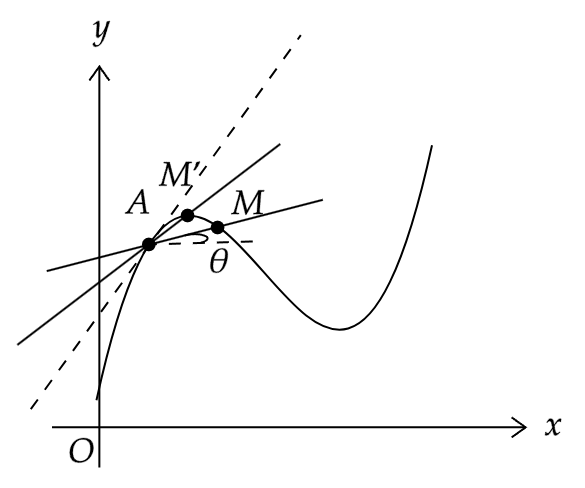
\includegraphics[width=0.6\textwidth]{Slides/figure/cattuyen.png}
        \caption{Cát tuyến của đồ thị hàm số}
    \end{figure}
    \end{column}
        \begin{column}{0.5\textwidth}
    Từ hình vẽ, ta thu được:
    \begin{equation}
    \tan\theta=\dfrac{f(x_M)-f(x_A)}{x_M-x_A}
    \end{equation}
    Khi lấy một điểm \(M'\) gần điểm \(A\) hơn \(M\) trên đồ thị, cát tuyến \(AM'\) sẽ gần với tiếp tuyến tại điểm \(A\) (đường nét đứt) hơn.
    \end{column}
    \end{columns}
\end{frame}
\begin{frame}{Đạo hàm}
    \begin{columns}
        \begin{column}{0.5\textwidth}
Khi điểm điểm \(M\) tiến gần đến điểm \(A\), độ dốc của cát tuyến \(AM\) sẽ tiến gần đến độ dốc của tiếp tuyến tại điểm \(A\):
\begin{figure}
    \centering
    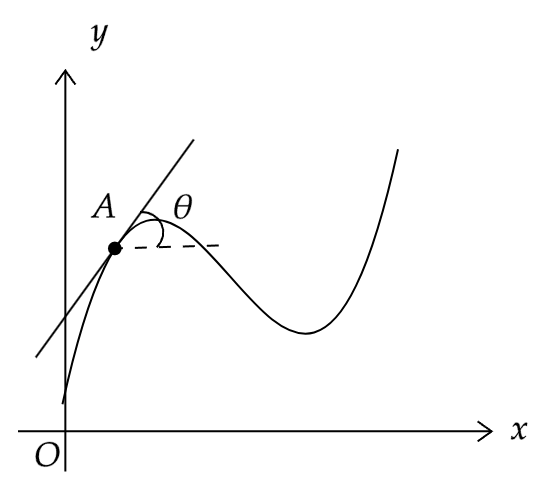
\includegraphics[width=0.6\textwidth]{Slides/figure/tieptuyen.png}
    \caption{Cát tuyến tiến gần đến tiếp tuyến}
\end{figure}
        \end{column}
        \begin{column}{0.5\textwidth}
Độ dốc của tiếp tuyến tại điểm \(A\) được tính bằng giới hạn:
\begin{equation}
    \tan\theta=\lim_{M\to A}\dfrac{f(x_M)-f(x_A)}{x_M-x_A}=f'(x_A)
\end{equation}
\(\longrightarrow\) Đạo hàm của hàm số tại điểm \(A\) phản ánh độ dốc của đồ thị tại điểm đó, cũng chính là tốc độ biến thiên của hàm số tại điểm đó.
        \end{column}
    \end{columns}
\end{frame}
\begin{frame}{Đạo hàm}
    Bảng đạo hàm của các hàm thông dụng:
    \begin{tcolorbox}[colback=blue!10, colframe=blue!50!black, title=]
    \begin{columns}
        \column{0.3\textwidth}
        \[
        \begin{aligned}
            &\dfrac{d}{dx}=nx^{n-1}\\
            &\dfrac{d}{dx}(\sin x)=\cos x\\
            &\dfrac{d}{dx}(\tan x)=\sec^2 x
        \end{aligned}
        \]
    \column{0.3\textwidth}
    \[
    \begin{aligned}
        &\dfrac{d}{dx}a^x=a^x \ln a\\
        &\dfrac{d}{dx}(\cos x)=-\sin x\\
        &\dfrac{d}{dx}(\cot x)=-\csc^2 x
        \end{aligned}
    \]
    \end{columns}
    \end{tcolorbox}
    \end{frame}